\documentclass[11pt,a4paper,english,final]{article}
\usepackage[english]{babel} % Using babel for norwegian hyphenation
\usepackage{lmodern} % Changing the font
\usepackage[utf8]{inputenc}
\usepackage[T1]{fontenc}

%\usepackage[moderate]{savetrees} % [subtle/moderate/extreme] really compact writing
\usepackage{tcolorbox}
\usepackage[parfill]{parskip} % Removes indents
\usepackage{amsmath} % Environment, symbols etc...
\usepackage{amssymb}
\usepackage{multirow} % For nice tables
%\usepackage{wasysym} % Astrological symbols
\usepackage{graphicx} % For pictures etc...
\usepackage{enumitem} % Points/lists
%\usepackage{physics} % Typesetting of mathematical physics examples: \bra{}, \ket{}, expval{}
\usepackage{url}

\definecolor{red}{RGB}{255,10,10}

% To include code(-snippets) with æøå
\usepackage{listings}
\lstset{
language=c++,
showspaces=false,
showstringspaces=false,
frame=l,
}

\tolerance = 5000 % Bedre tekst
\hbadness = \tolerance
\pretolerance = 2000

\numberwithin{equation}{section}

\newcommand{\conj}[1]{#1^*}
\newcommand{\ve}[1]{\mathbf{#1}} % Vektorer i bold
\let\oldhat\hat
\renewcommand{\hat}[1]{\mathbf{\oldhat{#1}}}
\newcommand{\trans}[1]{#1^\top}
\newcommand{\herm}[1]{#1^\dagger}
%\renewcommand{\thefootnote}{\fnsymbol{footnote}} % Gir fotnote-symboler
\newcommand{\Real}{\mathbb{R}}
\newcommand{\bigO}[1]{\mathcal{O}\left( #1 \right)}

\newcommand{\spac}{\hspace{5mm}}

\title{FYS3150/4150\\Computational Physics\\Project 1}
\author{Magnus Ulimoen\\Krister Stræte Karlsen}
\date{\today}

\begin{document}
\maketitle

\section{Introduction}

A great deal of differential equations in the natural sciences can be written 
as a linear second-order differential equation on the form
\begin{equation}
\frac{d^y}{dx^2} + k^2(x)y = f(x)
\label{eq:2orderDIFF}
\end{equation}


Some examples include
\begin{enumerate}[label=\bfseries \Roman*]
\item Schrödinger's equation
\item Airy function
\item Economics?
\item Poisson's equation
\item Laplace's equation (Poisson's with f=0)
\end{enumerate}

So being able to solve such equations optimally with respect to accuracy 
and efficiency is undoubtedly important. This report will compare 
different algorithms for solving them.

The algorithms to be investegated in this report is standard Gaussian Elemination, LU decomposition, sparse matrix decomposition and an algorithem specifically tailored for this problem. A tridiagonal system of linear equations. 


\subsection{A closer look at an example from Electromagnetism}

In electrostatics Maxwells equations reduces to
\begin{gather}
\nabla \cdot \ve{E} = \frac{\rho}{\epsilon_0}\\
\nabla \cdot \ve{B} = 0\\
\nabla \times \ve{E} = 0\\
\nabla \times \ve{B} = 0
\end{gather}
As the curl of the electric field is zero, the field is conservative
and can be written on the form
\begin{equation}
\nabla \Phi = -\ve{E}
\end{equation}
This gives Poisson's equation
\begin{equation}
\nabla^2\Phi = -\frac{\rho(\ve{r})}{\epsilon_0}
\end{equation}

Letting $\rho$ be spherically symmetric leads to a symmetric $\Phi$.
This gives with a substitution $\Phi(r) = \phi(r)/r$
\begin{equation}
\frac{d^2\phi}{dr^2} = -\frac{r\rho(r)}{\epsilon_0}
\end{equation}
Which is on the form of \eqref{eq:2orderDIFF}.

\section{Method}

The specific differential equation, with boundery values, being discussed in this report is: 

\begin{equation}
-u''(x) = f(x), \spac x \in (0,1), \spac u(0) = u(1) = 0.
\end{equation}

This boundery value problem can be discretized and written as a system of linear equations.

Letting the domain $x \in [0,1]$ be discretized into $n+1$ pieces,
\begin{gather}
x_0, x_1, \dots, x_i, \dots, x_{n+1}
\end{gather}
where 
\begin{gather}
h = \frac{x_{n+1} - x_0}{n+1} = \frac{x_{n+1}}{n+1}\\
x_i = x_0 + ih = ih
\end{gather}

an then sampling the solution at the mesh points so that $u(x_i) \simeq v_i$.

And using the three-point formula from the symmetric 
Taylor-expansion for the second derivative of v,
\begin{equation}
\frac{d^2v}{dx^2} \simeq \frac{v_{i-1} + v_{i+1} - 2v_i}{h^2}
\end{equation}

The discretized form of equation (2.1) can then be written as
\begin{gather}
\frac{v_{i-1} + v_{i+1} - 2v_i}{h^2} = \tilde{f}_i , \quad i=1,2, \dots, n 
\end{gather}
with $\tilde{f}_i = f(r_i) h^2$.

With boundary conditions 
\begin{gather}
v_0 = v_{N-1} = 0
\end{gather}

This can now be written as a system of linear equations on the form 

\begin{equation}
   \ve{A}\ve{v} = \tilde{\ve{b}},
   \label{eq:Avb}
\end{equation}

Multipling the discretized equation (2.6) by $h^2$ we get:

\begin{gather*}
   -v_{i-1}+2v_{i}-v_{i+1}=h^2 f_i \hspace{0.5cm} \mathrm{for} \hspace{0.5cm} i=1,\dots, n 
\end{gather*}

Filling in for $i$ and choosing $\tilde{b_i} = h^2 f_i$ we obtain the following set of equations: 
\begin{align*}
	2v_{1}-v_{2}=\tilde{b_1} \\
	-v_{1}+2v_{2}-v_{3}=\tilde{b_2} \\
	\vdots \hspace{0.5cm} \\
	-v_{i-1}+2v_{i}-v_{i+1}=\tilde{b_i} \\
	\vdots \hspace{0.5cm}  \\ 
	-v_{n-1}+2v_{n}=\tilde{b_n} \\
\end{align*}
Now one can easily see that this system of linear equations can written on the form of \eqref{eq:Avb}
\begin{gather*}
    \ve{A} = \begin{pmatrix}
                           2& -1& 0 &\dots   & \dots &0 \\
                           -1 & 2 & -1 &0 &\dots &\dots \\
                           0&-1 &2 & -1 & 0 & \dots \\
                           & \dots   & \dots &\dots   &\dots & \dots \\
                           0&\dots   &  &-1 &2& -1 \\
                           0&\dots    &  & 0  &-1 & 2 \\
                      \end{pmatrix},\spac \ve{v} = \begin{pmatrix}
                           v_1\\
                           v_2\\
                           \dots \\
                          \dots  \\
                          \dots \\
                           v_n\\
                      \end{pmatrix},
  \spac \tilde{\ve{b}} = \begin{pmatrix}
                           \tilde{b}_1\\
                           \tilde{b}_2\\
                           \dots \\
                           \dots \\
                          \dots \\
                           \tilde{b}_n\\
                      \end{pmatrix}.
\end{gather*}

Having a complete set of linear equations we move on to how to solve them.

\subsection{A tridiagonal matrix algorithm}
\label{subsec:Thomas}

We start by looking at the system of equations:
\begin{align}
	 b_1 v_1 + c_1 v_{2} = \tilde{b_1} \label{eq:1star}\\
	 a_2 v_1 + b_2 v_2 + c_3 v_3 = \tilde{b_2} \label{eq:2star}\\
	 a_3 v_2 + b_3 v_3 + c_3 v_4 = \tilde{b_3} \label{eq:3star}\\
\nonumber\vdots \hspace{0.5cm}  \\ 
	 a_n v_{n-1} + b_n v_n = \tilde{b_n} \label{eq:Nstar}
\end{align}
If we solve \eqref{eq:1star} for $v_1$ and insert it into \eqref{eq:2star} we obtain the following "modified second equation":
\begin{align*}
	(b_1 b_2 - a_2 c_1)v_2 + b_1 c_2 v_3 = b_1 \tilde{b_2} - a_2  \tilde{b_1}  
\end{align*}
Now having successfully removed $v_1$ from the second equation we can go on and solve it for $v_2$ and insert it into the third equation obtaining:
\begin{align*}
(b_3 (b_1 b_2 - a_2 c_1)- a_3 b_1 c_2)v_3 + c_3(b_1 b_2 -a_2 c_1)v_4 = \\
(b_1 b_2 - a_2 c_1 ) \tilde{b_3} - a_3 b_1 \tilde{b_2} + a_2 a_3 \tilde{b_1} 
\end{align*}

The two modified equations may be written as 

\begin{align*}
v_2 = \frac{b_1 \tilde{b_2} - a_2 \tilde{b_1}}{b_1 b_2 - a_2 c_1} - \frac{b_1 c_2}{b_1 b_2 - a_2 c_1} v_3 = \beta_2 + \gamma_2 v_3
\end{align*}
\begin{align*}
v_3 =& \frac{(b_1 b_2 - a_2 c_1) \tilde{b_3} - a_3 (b_1 \tilde{b_2} - a_2 \tilde{b_1})}{b_3 (b_1 b_2 - a_2 c_1)- a_3 b_1 c_2} - \frac{c_3(b_1 b_2 - a_2 c_1)}{b_3 (b_1 b_2 - a_2 c_1)- a_3 b_1 c_2} v_4 \\
=&  \frac{\tilde{b_3}-a_3 \beta_2}{a_3 \gamma_2 + b_3} + \frac{-c_3}{a_3 \gamma_2 + b_3}v_4 = \beta_3 + \gamma_3 v_4
\end{align*}

This prossess can be repeated up untill the last equation. 
This is the forward substitution step. 
From the last equation we compute $v_n$ and get all we need to compute $v_{n-1}$,
then $v_{n-2}$, and so on. This is the backward substitution part of the algorithm. A shrewd reader might see that the coefficiants, $\beta$ and $\gamma$, take a recursive form
\begin{align*}
\beta_{i} = \frac{\tilde{b_i}-a_i \beta_{i-1}}{a_i \gamma_{i-1} + b_i} , \hspace{0.5cm} \gamma_{i}=\frac{-c_i}{a_i \gamma_{i-1} + b_i},
\end{align*}
and the equation for $v_{i-1}$ reads: 
\begin{equation}
v_{i-1} = \beta_{i-1} + \gamma_{i-1} v_i
\label{eq:viminus1}
\end{equation}

It follows from \eqref{eq:1star} that $\beta_1 = \frac{\tilde{b_1}}{b_1}$ and $\gamma_1 = \frac{-c_1}{b_1}$.
From combining \eqref{eq:Nstar} and \eqref{eq:viminus1} we get 
\begin{align*}
v_n = \frac{\tilde{b_n}-a_n \beta_{n-1}}{a_n \gamma_{n-1} + b_n} = \beta_{n}.
\end{align*}

Having all the nessecary ingredients the algorithm reads as follows.
\vspace{0.5cm}

\centerline{Algorithm I}
\begin{tcolorbox}
$a_i = c_i = -1, \hspace{0.5cm}  i=1,2,3,..,n$\\
$b_i = 2, \hspace{0.5cm}  i=1,2,3,..,n $\\
$\tilde{b_i} = h^2 f_i \hspace{0.5cm}  i=1,2,3,..,n $\\
$\beta_1 = \frac{\tilde{b_1}}{b_1}$ \\
$\gamma_1 = \frac{-c_1}{b_1}$ \\
for $i=2,3,..,n$ \\ \vspace{0.5cm} 
 \hspace{0.5cm} $ \beta_{i} = \frac{\tilde{b_{i-1}}-a_{i-1} \beta_{i-1}}{a_{i-1} \gamma_{i-1} + b_{i-1}} , \hspace{0.5cm} \gamma_{i}=\frac{-c_{i-1}}{a_{i-1} \gamma_{i-1} + b_{i-1}} $ \vspace{0.2cm}  \\
 $v_{n} = \beta_{n}$\\
for $i=n, n-1, \cdots ,2$\\ \vspace{0.5cm} 
 \hspace{0.5cm} $v_{i-1} = \beta_{i-1} + \gamma_{i-1} v_i$
\end{tcolorbox} 


This is often refered to as \emph{Thomas Algorithm}, an algorithm for solving tridiagonal systems of linear equations. 

\subsubsection{Implementation}

The algorithm in section \ref{subsec:Thomas} is implemented in C++.
This requires three arrays to be created, which holds $\beta_i$, $\gamma_i$
and $\tilde{f}_i$. These arrays are zero-indexed, and the implementation
follows this.

Our implementation assumes constant a, b, c, and the elements $a_i$
used in the algorithm is not implemented in the code. This is 
easily changed for more general purposes.

\subsection{Standard Gaussian Elimination}

The Gaussian elimination is solving the system \eqref{eq:Avb} by using 
row operations and getting a row echelon form and then backsubstituting.

A matrix
\begin{gather}
A = \begin{pmatrix}
    a_{11} & a_{12} & a_{13} & \cdots\\
    a_{21} & a_{22} & a_{23} & \cdots\\
    a_{31} & a_{32} & a_{33} & \cdots\\
    \cdots \\
    a_{n1} & a_{n2} & \cdots
    \end{pmatrix}
\end{gather}

To get the matrix into the row echelon the first row needs to have a non-zero
value as its first element. Then a constant $c_i = a_{i1}/a_{11}$ is 
calculated, and a subtraction of the first row,
\begin{gather}
a_{ij} = a_{ij} - c_i a_{ij}
\end{gather}
is done. For the elements $a_{i1}$, this gives zero, and the matrix is
row reduced to
\begin{gather}
A \sim
\begin{pmatrix}
    a_{11} & a_{12} & a_{13} & \cdots\\
    0 & a_{22} - c_2 a_{22} & a_{23} - c_2 a_{23} & \cdots\\
    0 & a_{32} - c_3 a_{32} & a_{33} - c_3 a_{33} & \cdots\\
    0 & \cdots \\
    0 & a_{n2} - c_2 a_{n2} & \cdots
\end{pmatrix}
\end{gather}
The operation can be repeated on the submatrix $A_{(2-N)(2-N)}$
until the decired triangular matrix is achieved.

The backsubstitution is simple when a row reduced matrix is achieved,
by looking at the matrix equation $Ux = y$
\begin{gather}
\begin{pmatrix} u_{11} & u_{12} & \dots\\
                0 & u_{22} & u_{23} & \dots\\
                &\dots & \dots\\
                0 & \dots & a_{(n-1)(n-1)} & a_{(n-1)n} \\
                & \dots & 0 & a_{nn}
\end{pmatrix} \begin{pmatrix} x_1 \\ x_2 \\ \dots \\ x_{n-1}\\ x_n \end{pmatrix}
 = \begin{pmatrix} y_1 \\ y_2 \\ \dots\\ y_{n-1} \\ y_n \end{pmatrix}\\
 x_n = \frac{y_n}{a_{nn}}\\
 x_{n-1} = \frac{y_{n-1} - a_{(n-1)n}x_n}{a_{(n-1)(n-1)}}
\end{gather}
Where $x_{i}$ is found from a recursive method.

\subsubsection{Implementation}

The matrix solvers are used from the Armadillo 
library\footnote{\url{http://arma.sourceforge.net/}}. The matrix is
created by indexing the non-zero elements and setting this equal to the 
tridiagonal elements. The calculation is done by a call to 
\begin{lstlisting}
arma::Col<double> x = solve(A, b);
\end{lstlisting}


\subsection{LU decomposition}

When the matrix equation \eqref{eq:Avb} is solved, this is modified into
an upper triangular and lower triangular matrix. The lower matrix (L) 
diagonal has elements with the value 1, and is invertible if A is 
non-singular.

The LU decomposition allows one to find the sets of linear equations,
\begin{gather}
Ax = LUx = w
\end{gather}
Is then solved for x by using a the inverse of L (which exist due to its 
construction), 
\begin{gather}
Ux = L^{-1}w = y
\end{gather}
Since U is an upper triangular matrix the solution is found from back-substitution
of the elements as described in the Gaussian Elimination.

\subsubsection{Implementation}

\textcolor{red}{KSK: Implementation of LU to be added here.}

\subsection{Method using sparse}

To prevent saving a very sparse matrix in memory a sparse method can be employed.
This saves the non-zero matrix elements and location instead of the 
entire matrix. This saves memory and computational speed, as only these
elements are manipulated.

\subsubsection{Implementation}

The matrix solution above is very ineffective in both the amount
of computations and memory usage. This is improved by using sparse 
matrices, which saves the non-zero elements by position and value.

For our very sparse matrix which has $N-3$ unused elements per row, the
memory-space saved is $(N-3)^2$. This helps keep the matrix in the 
CPU-cache and speeds it up for larger matrices.

The calculation is done by a call to
\begin{lstlisting}
arma::Col<double> x = spsolve(spA, b);
\end{lstlisting}

\section{Results}

\subsection{Speed/Efficiency}

\begin{center}
\textbf{Table 1}: Comparing the time, number of clock cycles per MHz for the different algorithms for different number of mesh points.  

\begin{tabular}{|l|l|l|l|l|l|l|l|}
\hline
\multicolumn{1}{|c|}{ } & \multicolumn{1}{|c|}{Gauss Elimination} & \multicolumn{1}{|c|}{TDMA.} & \multicolumn{1}{|c|}{Sparse decompostion} & \multicolumn{1}{|c|}{LU decomposition}  \\
\hline
N & Time & Time & Time & Time  \\
\hline
10 & 4.42000000e-04 &   2.50000000e-05 &   5.32000000e-04 & 1.86820000e-02 \\
25 & 5.09000000e-03 &   3.40000000e-05 &   8.06000000e-04 & 5.11400000e-03 \\
50 & 5.94300000e-02 &   7.70000000e-05 &   8.18000000e-04 & 1.01090000e-02 \\
100 & 3.55500000e-03 &   4.80000000e-05 &   1.14700000e-03 & 1.07380000e-02 \\
250 & 1.72380000e-02 &   1.19000000e-04 &   2.66800000e-03 & 8.30680000e-02 \\
500 & 2.83505000e-01 &   2.08000000e-04 &   8.02000000e-03 & 2.14431000e-01 \\
1000 & 3.55766000e-01 &   3.66000000e-04 &   1.68560000e-02 & 1.31517900e+00 \\
2000 & 1.75258000e+00 &   9.27000000e-04 &   7.37350000e-02 & 9.11888400e+00 \\
3000 & 4.48197300e+00 &   1.14700000e-03 &   2.08975000e-01 & 2.39678190e+01 \\
4000 & 1.01286820e+01 &   1.87500000e-03 &   2.66886000e-01 & 5.86866600e+01 \\
5000 & 1.93415310e+01 &   2.37900000e-03 &   3.97806000e-01 & 1.08909192e+02 \\
6000 & 3.20998800e+01 &   2.22900000e-03 &   5.35781000e-01 & 1.89079185e+02 \\
\hline
\end{tabular}
\end{center}

\begin{figure}[h!]
\centering
  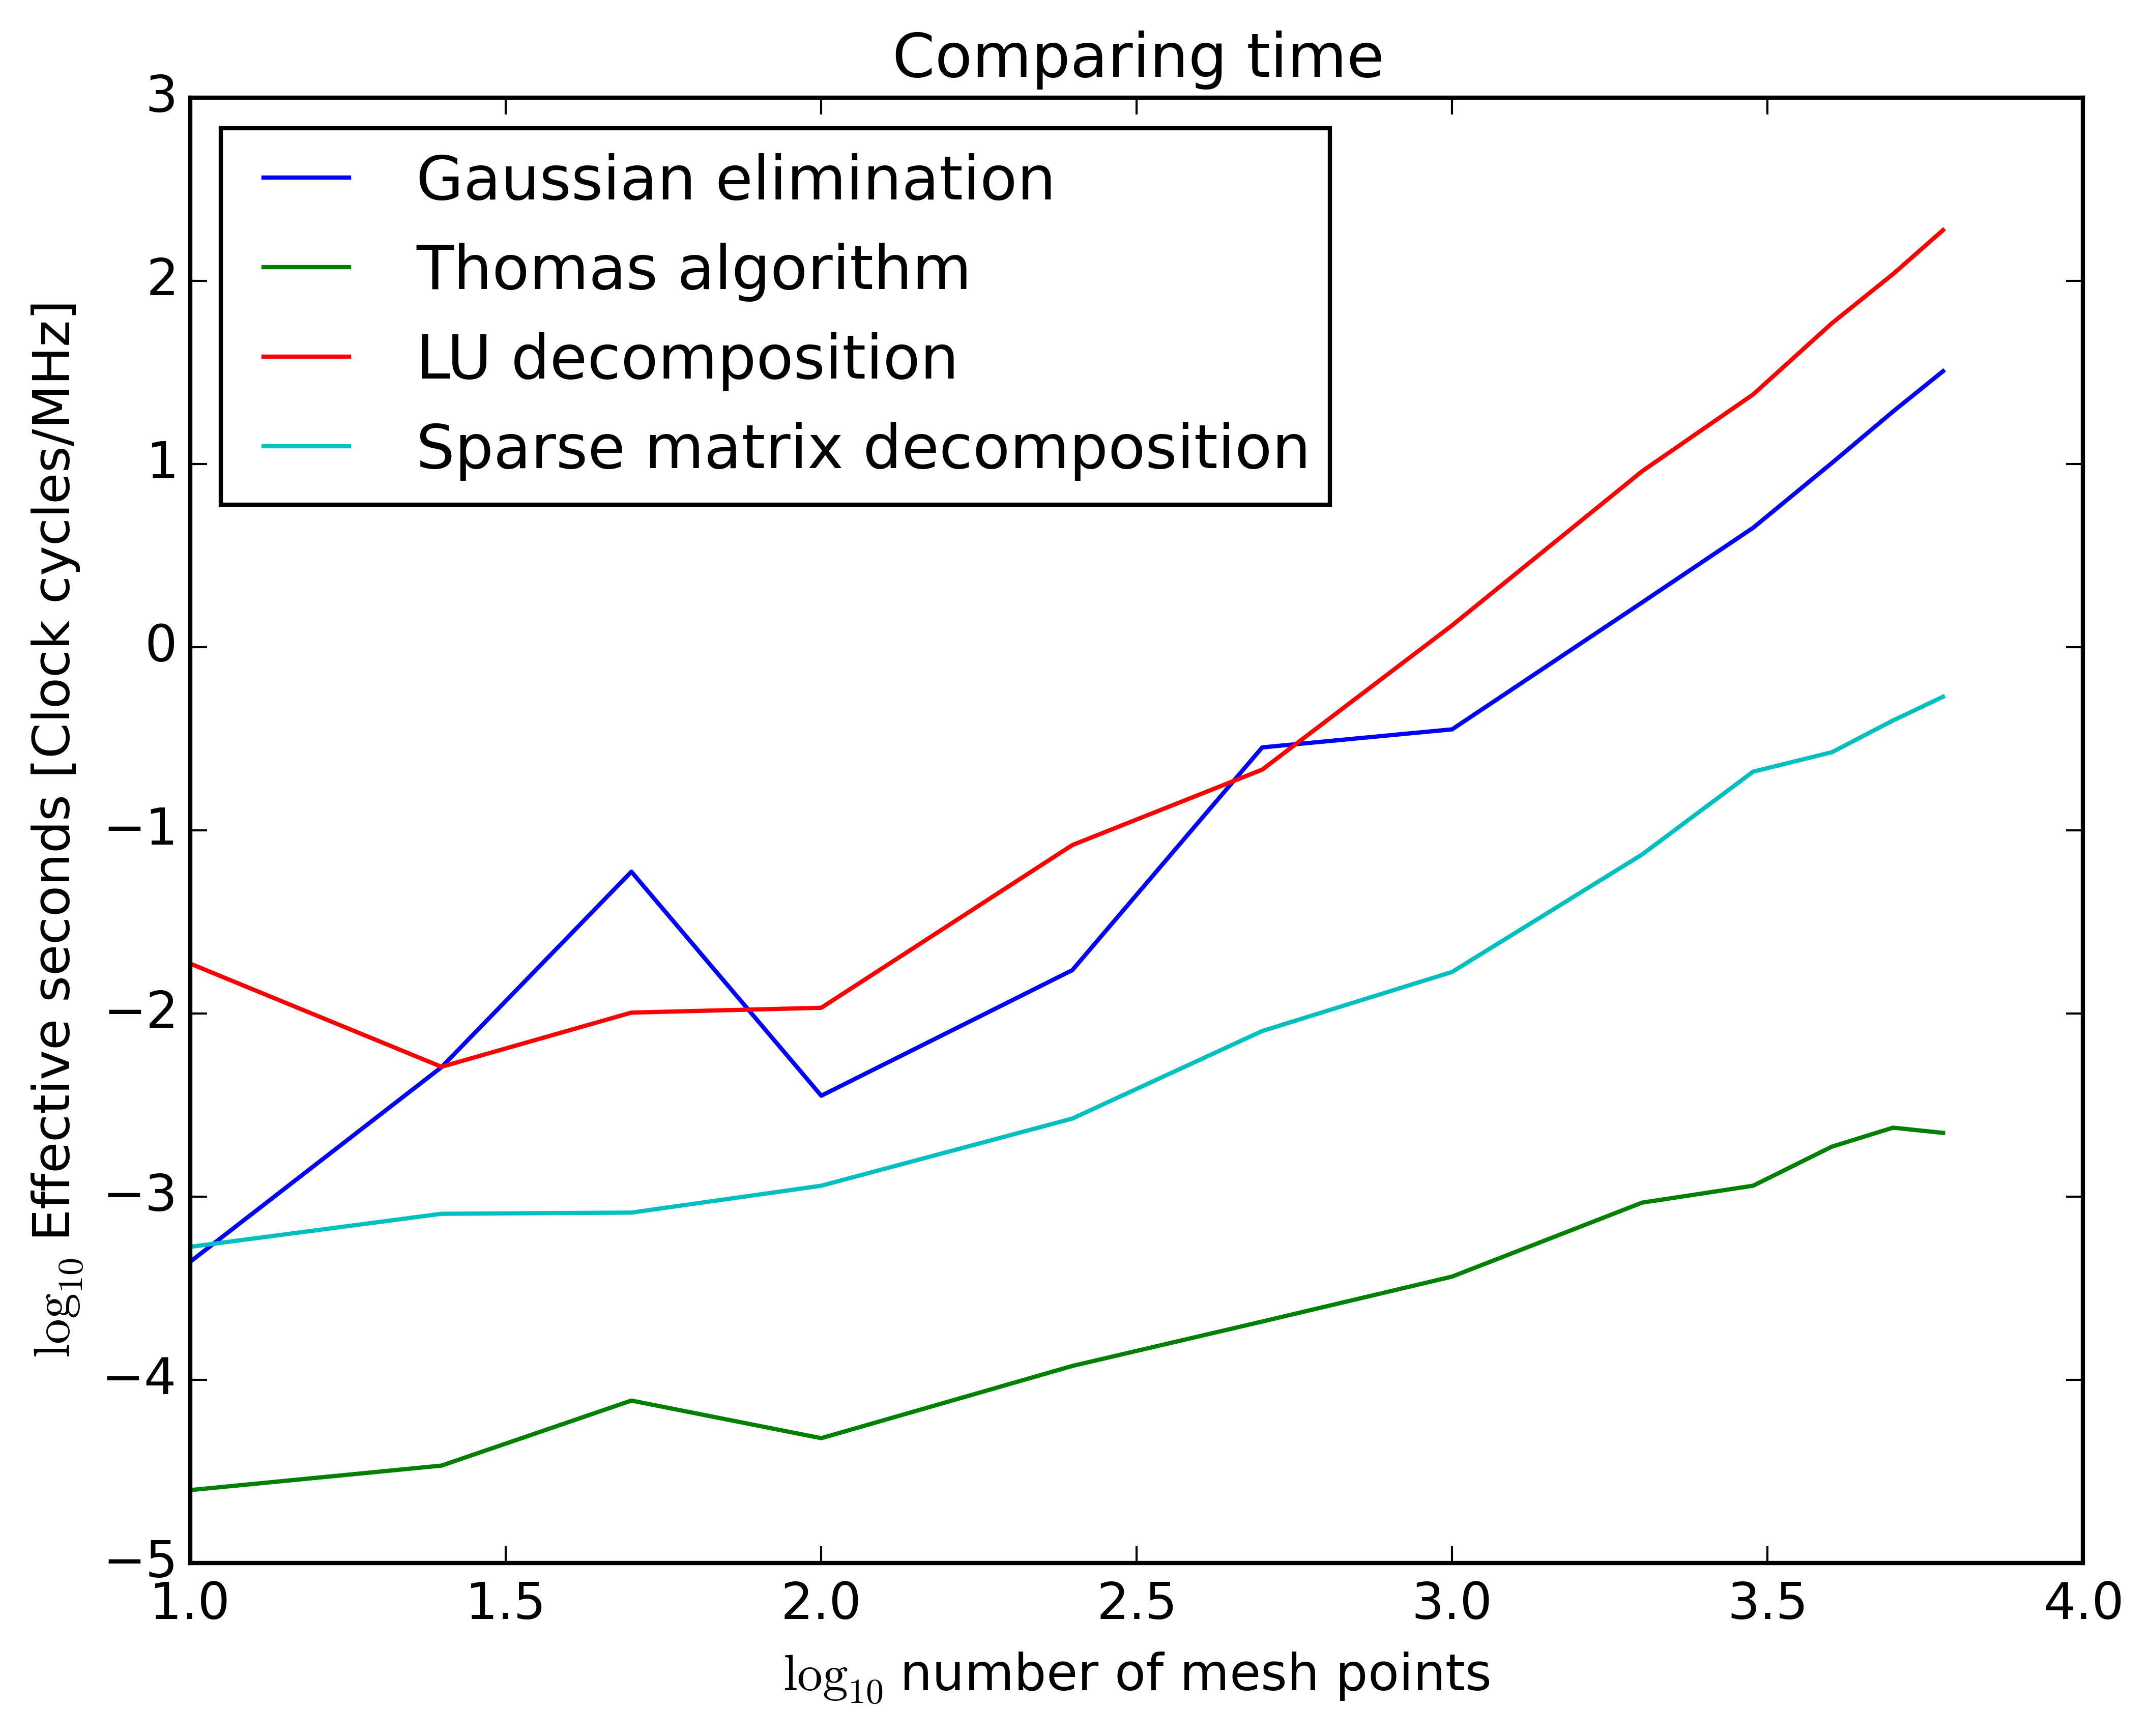
\includegraphics[scale=0.5]{n_time.png}
  \caption{Insert some meaningful caption here. }
\end{figure}


\subsection{Accuracy/Error}

\begin{figure}
\textbf{Table 2}: Comparing accuray of different algorithms for a different number of mesh points. The error here is defined as $log_{10}$ of the maximum relative error. 

\begin{tabular}{|l|l|l|l|l|l|l|l|}
\hline
\multicolumn{1}{|c|}{ } & \multicolumn{1}{|c|}{Gauss Elimination} & \multicolumn{1}{|c|}{TDMA.} & \multicolumn{1}{|c|}{Sparse decompostion} & \multicolumn{1}{|c|}{LU decomposition}  \\
\hline
N & Error & Error & Error & Error  \\
\hline
10 & 0.34469208 &  0.34469208 &  0.34469208 &  0.34469208\\
25 & 0.14844317 &  0.14844317 &  0.14844317 &  0.14844317\\
50 & 0.07648232 &  0.07648232 &  0.07648232 &  0.07648232\\
100 & 0.0388765  &  0.0388765  &  0.0388765  &  0.0388765 \\
250 & 0.01571379 &  0.01571379 &  0.01571379 &  0.01571379\\
500 & 0.00788507 &  0.00788507 &  0.00788507 &  0.00788507\\
1000 & 0.00394968 &  0.00394968 &  0.00394968 &  0.00394968\\
2000 & 0.00197664 &  0.00197664 &  0.00197664 &  0.00197664\\
3000 & 0.00131816 &  0.00131816 &  0.00131816 &  0.00131816\\
4000 & 0.00098877 &  0.00098877 &  0.00098877 &  0.00098877\\
5000 & 0.00079109 &  0.00079109 &  0.00079109 &  0.00079109\\
6000 & 0.00065928 &  0.00065928 &  0.00065928 &  0.00065928\\
\hline
\end{tabular}
\end{figure}

\begin{figure}[h!]
\centering
  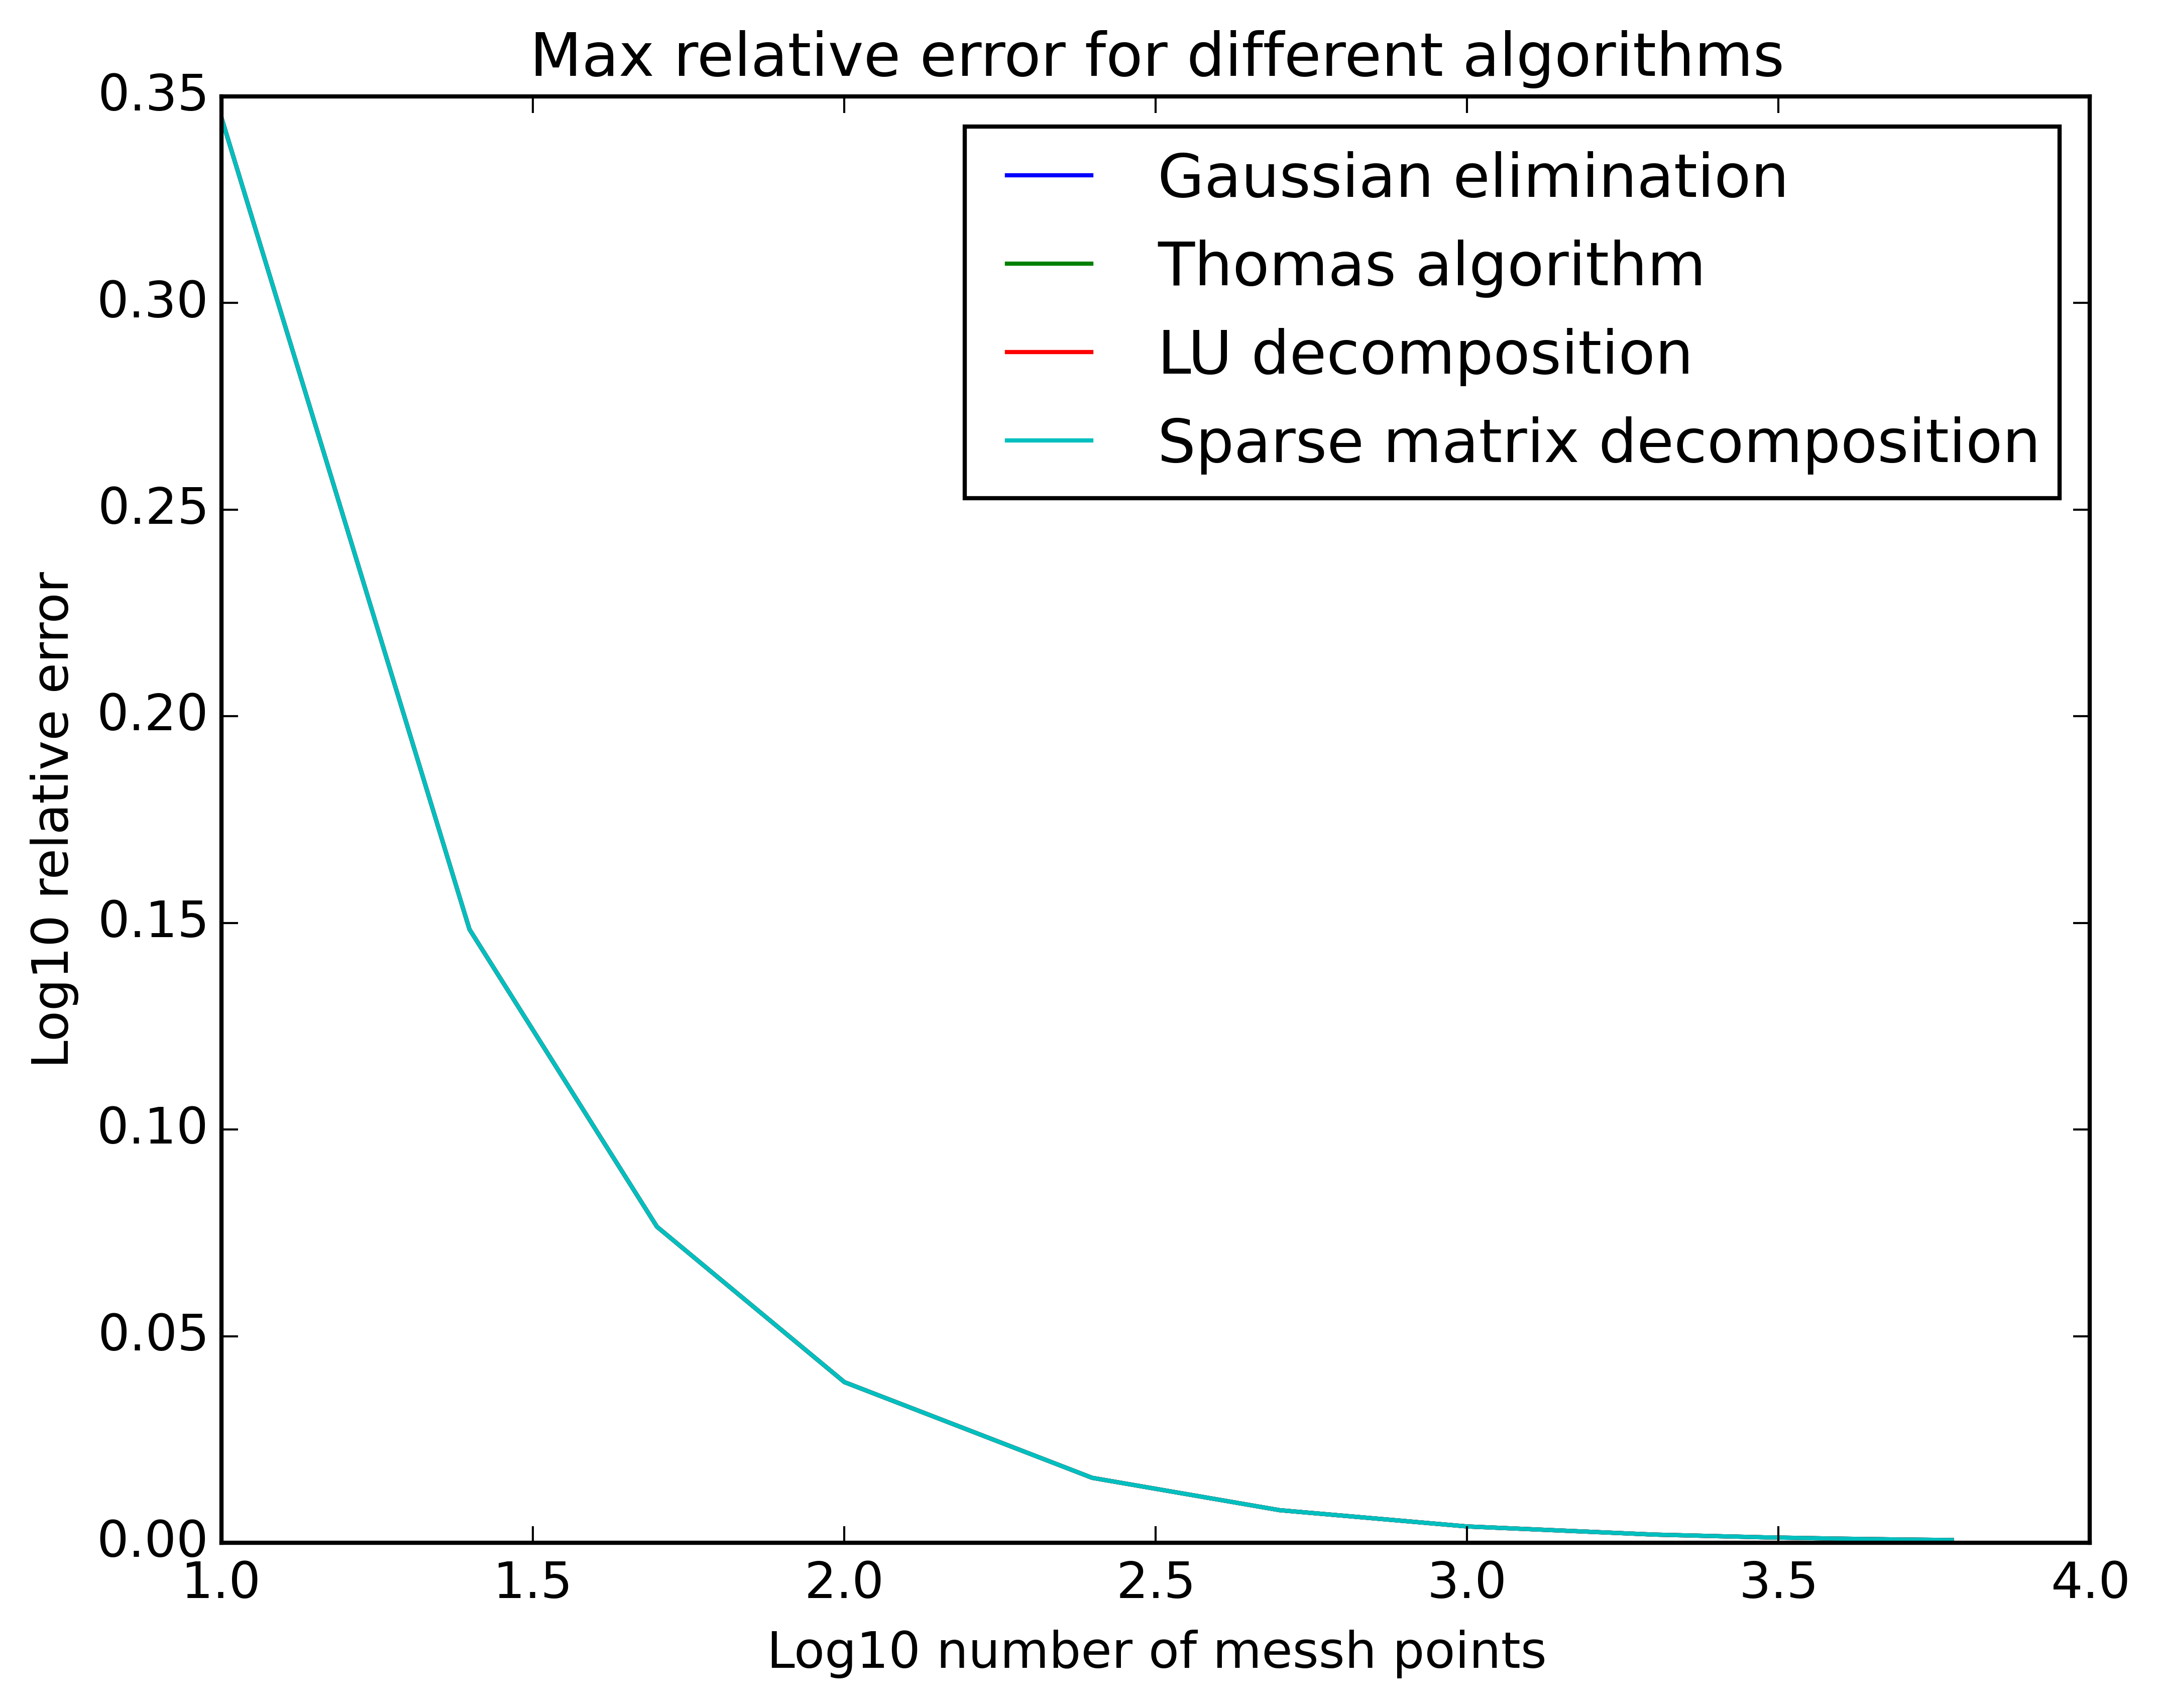
\includegraphics[scale=0.5]{n_err.png}
  \caption{Insert some meaningful caption here. }
\end{figure}


\subsection{FLOPS}

The number of floating point operations (FLOPS) per algorithm gives a useful 
metric of the scalability. The more FLOPS required the more time is
required for larger systems. This is usually given in $\bigO{x}$ notation,
where x gives approximately the number of calculations.

\subsubsection{Thomas algorithm}
This algorithm requires nine operations for each row for the forward substitution,
and two backwards. This requires 11 FLOPS for each row to solve the system.
With n rows this algorithm requires 11N FLOPS.

In big O notation the complexity of $\bigO{n}$.

\subsubsection{Gaussian decomposition}
For a general matrix with size ($N\times N$), the algorithm requires
$N^2$ operations per row reduction. This is repeated for all N rows,
and the complexity is $\bigO{n^3}$ for the reduction. The backwards 
substitution has $\bigO{n^2}$ and is not of significance.

For a sparse matrix (with suitable algorithms) this could be less, 
as some of the row operations are
skipped. This leads to a lower amount of FLOPS needed for a sparse
matrix.

\subsubsection{LU decomposition}
The decomposition into the LU-matrix requires $\bigO{N^3}$ FLOPS, but 
has the advantage that backwards substitution just requires $\bigO{N^2}$
FLOPS to compute. This decomposition is also highly reusable if \eqref{eq:Avb}
is to be solved for more than one $\ve{x}$, or the determinant is to be found.

\section{Discussion}

Can solve the equation \eqref{eq:Avb} directly by LU-decomposition.
The matrix A is then transformed into one upper triagonal matrix and
one lower diagonal matrix. By doing this on a matrix this results in an
easier way to solve several $Ax = y$ for different y.

Direct solver by arma::solve(A, y) is used to compare with the LU-method.
This is ordinary quicker, since armadillo is a high-level wrapper around
lapack etc.

\subsection{FLOPS}
The standard is $\bigO{N^3}$ complexity

\section{Concluding remarks}


We see that the algorithm developed in section \ref{subsec:Thomas} is 
well suited for this problem.


\end{document}
